%!TEX root = main.tex
\section{Data samples}
\begin{frame}
\frametitle{Data samples}
For Pb-Pb collisions
\begin{itemize}
		\item{Pb-Pb : LHC10h and 11h at $\sqrt{s_\mathrm{NN}}$ = 2.76 TeV}
		\item{MC for correction : LHC12a15e$\_$fix (PYTHIA6$-$2011)}
\end{itemize}


For p-Pb or Pb-p collisions
	\begin{itemize}
		\item{p-Pb : LHC13 d and e $\sqrt{s_\mathrm{NN}}$ = 5.02 TeV}
		\item{Pb-p : LHC13 f $\sqrt{s_\mathrm{NN}}$ = 5.02 TeV }
		\item{MC for correction : LHC13b4$\_$fix and LHC13b4$\_$plus (PYTHIA6$-$2011)}
	\end{itemize}
	
For pp collisions
	\begin{itemize}
	         \item{pp : LHC12h  $\sqrt{s}=8$ TeV}
	         \item{MC for model and correction : LHC16c2 (PYTHIA8)}
	\end{itemize}

\end{frame}

\begin{frame}
\frametitle{Event and track selection}
Trigger selection : kEMCJE 
\begin{itemize}
\item Trigger bias existing
\item all observables ($\mathrm{d}N/\mathrm{d}M_\mathrm{jj}$ ,$\mathrm{d}N/\mathrm{d}p_\mathrm{T,pair}$ ) are scaled to INT7 by $\frac{\mathrm{d}N/\mathrm{d}p_\mathrm{T,jet}^{\textrm{INT7, LHC13b or c}}}{\mathrm{d}N/\mathrm{d}p_\mathrm{T,jet}^{\textrm{EMCJE, LHC13 d, e or f}}}$
\end{itemize}
Vertex cut : $|z_\mathrm{vtx}|<10$ cm\\

Track selection : Hybrid tracks for primary track selection\\

Jet reconstruction algorithm : anti-kt\\
Jet selection 
	\begin{itemize}
	\item{charged jets in the TPC acceptance reconstructed by the EMCAL framework }
	\item{$p_\mathrm{T}^\mathrm{leading\,particle}>$ 5 GeV/$c$}
	\item{R $=$ 0.4}
	\end{itemize}
	
Dijet selection 
	\begin{itemize}
		\item{ $p_\mathrm{T}^{\textrm{leading jet}}$ $>$  $p_\mathrm{T}^{\textrm{sub-leading jet}}$ $>$ 20 GeV/$c$}
	\end{itemize}

\end{frame}

	
\begin{frame}
\frametitle{Invariant mass of charged jets}
Jet-axis reconstruction scheme : pt-scheme (four momentum sum of associated particles)
\begin{itemize}
	\item{$M^{\textrm{tracks}\in \textrm{cone}}$ = 0}
	\item{$E = |\vec{p}|$}
\end{itemize}
How to give invariant mass to a jet
\begin{itemize}
	\item {$E^{\textrm{tracks} \in \textrm{cone}}$ are recalculated such that $M^{\textrm{tracks}\in \textrm{cone}}$ = pion mass} (pion-mass assumption)
\end{itemize}
\end{frame}

\begin{frame}

\frametitle{Unfolding}
Detector efficiency are corrected by multi-dimensional unfolding method
\begin{itemize}
\item{Package : RooUnfold}
\item{Algorithm : Iterative}
\end{itemize}

	\begin{equation}
	%\mathrm{Raw}(M_\mathrm{dijet},p_\mathrm{T,pair}) \times \frac{\mathrm{MC truth}(M_\mathrm{dijet},p_\mathrm{T,pair})}{\mathrm{MC rec}(M_\mathrm{dijet},p_\mathrm{T,pair})}
	(M_\mathrm{jj}^\mathrm{raw},p_\mathrm{T,jj}^\mathrm{raw}) \times \mathcal{R} (M_\mathrm{jj}^\mathrm{mcrec},M_\mathrm{jj}^\mathrm{mctrue},p_\mathrm{T,jj}^\mathrm{mcrec},p_\mathrm{T,jj}^\mathrm{mctrue})
	\end{equation}
Corrected $(M_\mathrm{jj}^\mathrm{corrected},p_\mathrm{T,jj}^\mathrm{corrected})$ 
\begin{itemize}
\item{projection on $M_\mathrm{jj}$ axis}
\item{projection on $p_\mathrm{T,jj}$ axis for different $M_\mathrm{jj}$ bin ranges}
\end{itemize}	

\end{frame}

\begin{frame}
\frametitle{Unfolding - closure test}
Closure test for the unfolding with MC samples
\begin{columns}[t]
\column{.5\textwidth}
\centering
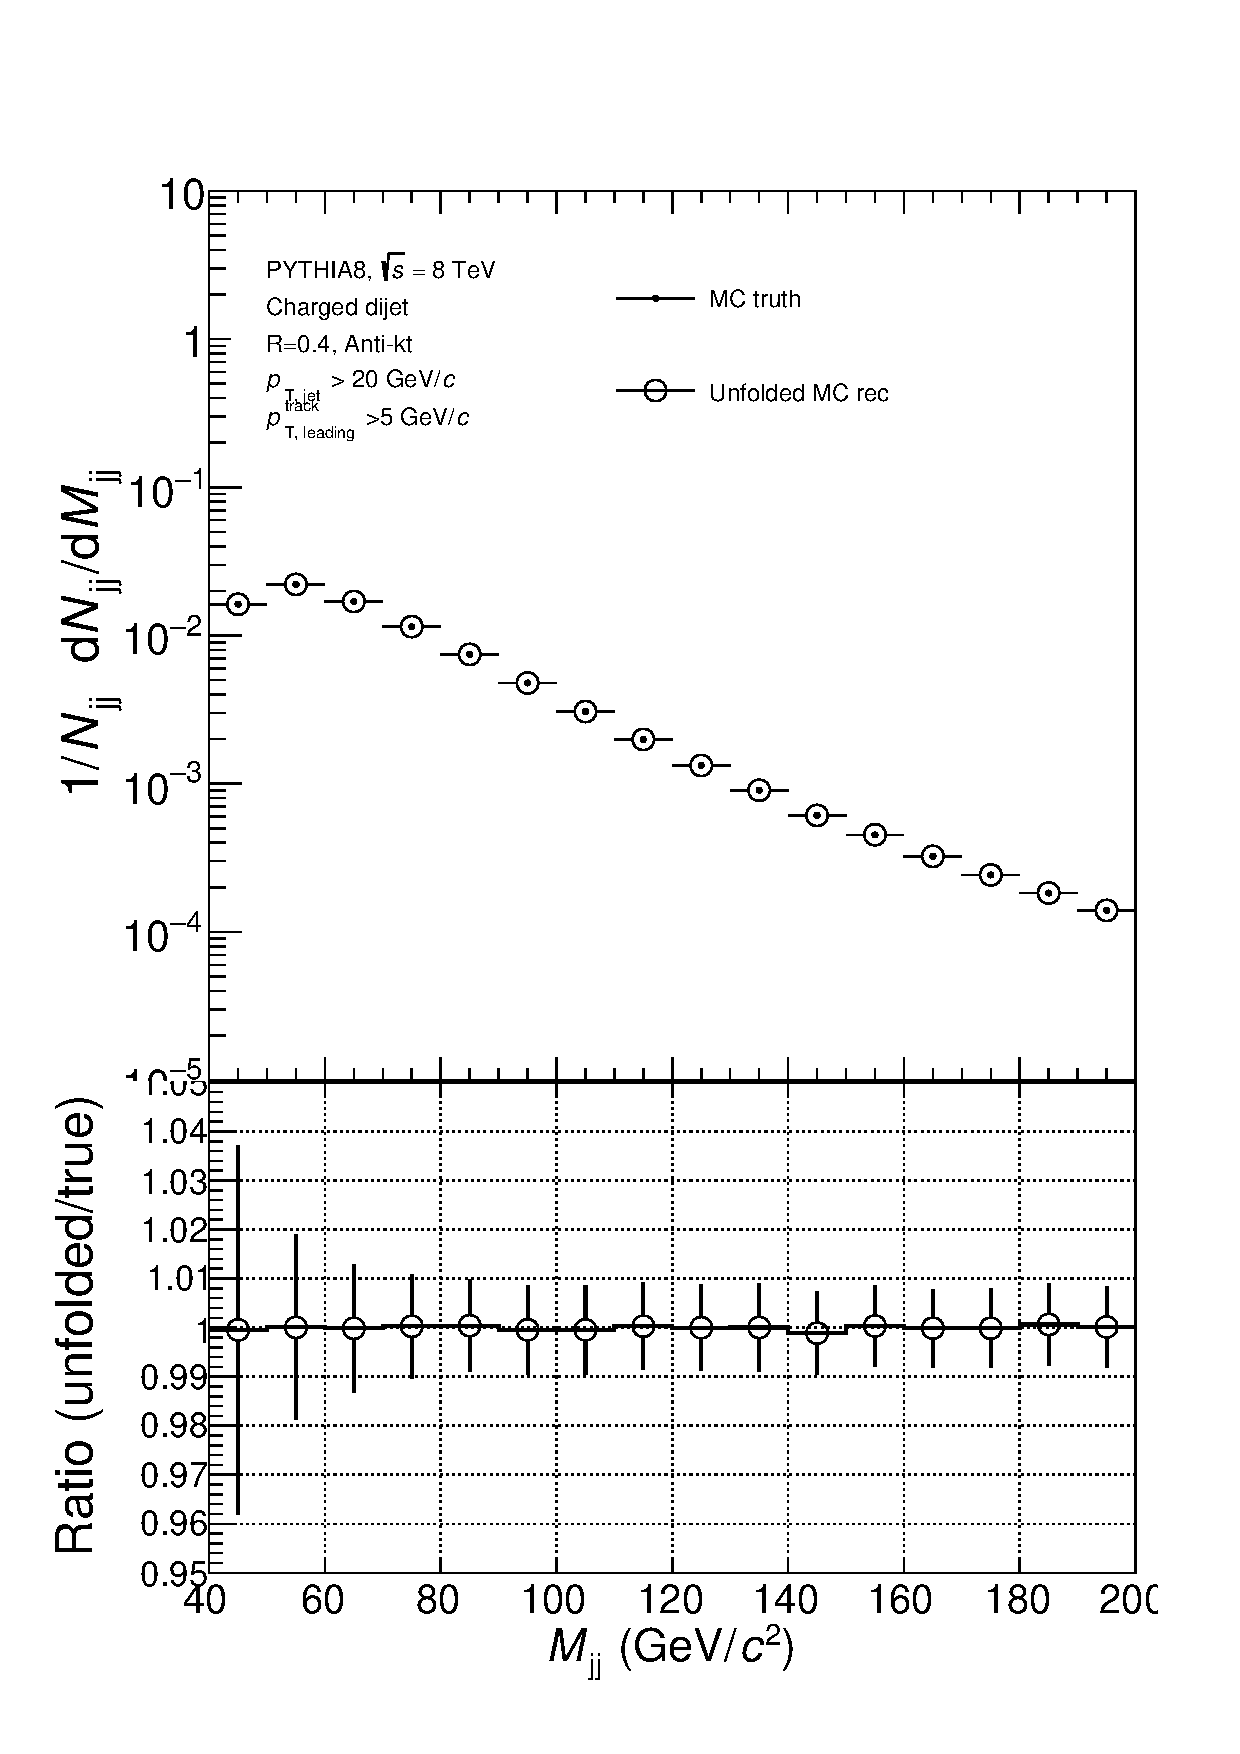
\includegraphics[width=1\linewidth]{mjj_closure}\\
\column{.5\textwidth}
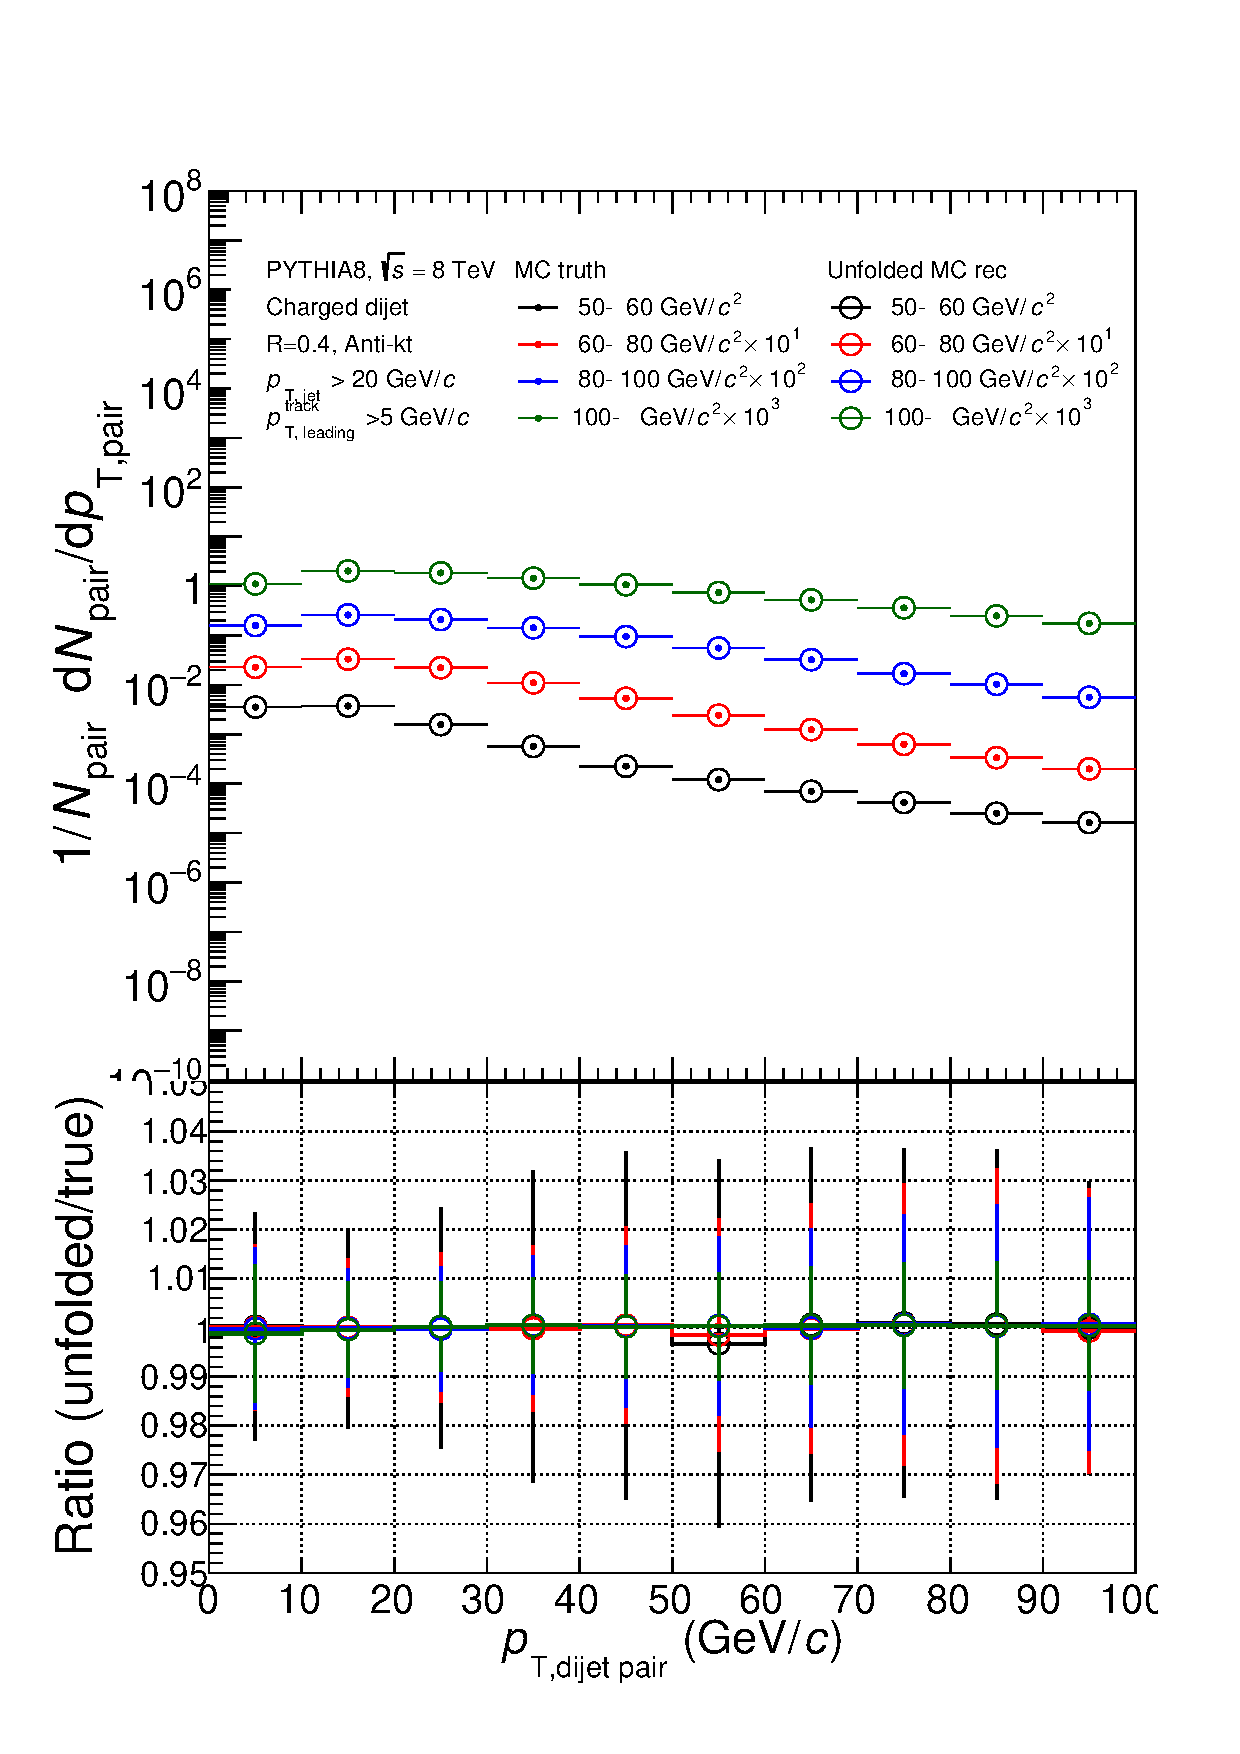
\includegraphics[width=1\linewidth]{ptjj_closure}\\
\end{columns}
\end{frame}




















